
\section{Punktoperation und Bildverknüpfungen}
Bei den Punktoperationen wird jedes Pixel isoliert betrachtet und unabhängig von seinen Nachbarpixel verändert.
\subsection{Transformationstabellen}
Es wird grundsätzlich zwischen zwei verschiedenen Arten unterschieden:
\begin{description}
    \item[Homogene Punktoperationen] Bei diesen Operationen spielt die Position des Pixels keine Rolle für die angewendete Transformation.\\
    Bsp. Invertiertes Bild
    \item[inhomogene Punktoperationen] Bei dieser Art von Operationen wird die Position des Pixels für die Transformation berücksichtigt.\\
    Bsp. Farbverlauf
\end{description}

\subsubsection{Lineare Grauwerttransformationen}
Beispiele sind: \textbf{Spreizung} und \textbf{inverses Bild}\\
Für lineare Transformationen werden oft LUT (Look up tables) verwendet.
\begin{lstlisting}
%LUT for inverse image
LUT_Inv = uint8([255:-1:0]);

% LUT for spreading (Spreizung)
LUT_Spread = uint8(((0:255)-50) * 2);

%apply LUT
ImageInv = intlut(Image, LUT_xx);
\end{lstlisting}

\subsubsection{Nichtlineare Grauwerttransformationen (Gammakorrektur)}
Wichtigstes Beispiel: \textbf{Gammakorrektur}
Die Gammakorrektur ist eine häufig verwendete Korrekturfunktion zur Überführung einer physikalisch proportional (d. h. linear) wachsenden Grösse in eine dem menschlichen Empfinden gemäss nicht linear wachsende Grösse.

\subsection{Histogrammausgleich}
Der Histogrammausgleich versucht den zur Verfügung stehenden Grauwertbereich optimal auszunutzen. Dabei sollte jeder Grauwert gleichmässig auftreten.
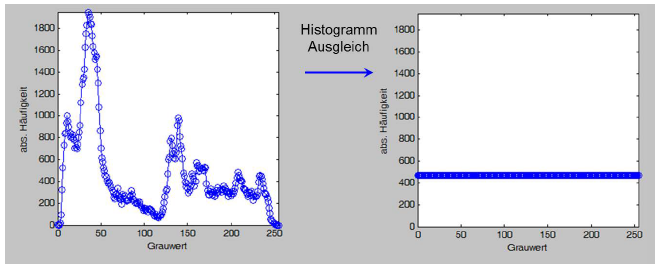
\includegraphics[width=\textwidth/3]{histogrammausgleich.PNG}
\begin{lstlisting}
[Hist, Val] = imhist(Image);

CumHist = cumsum(Hist)/sum(Hist);
% remark: cumsum()
% Addiert alle Ellemente von 0 bis i.

%do the histogram equalization
%LUT for histogram equalization
LUT_Equ = uint8(CumHist*255);

%apply LUT
ImageEqu = intlut(Image, LUT_Equ);
\end{lstlisting}

\subsection{Motiondetektion durch Differenzbildung}
Durch Substraktion von zwei Bildern kann die Veränderung zwischen den Bildsequenzen erkennt werden.
\begin{lstlisting}
%this is the delta of the step
Delta = 2;

%read first image to index 0
Index = 0;
FileName = strcat(Path, sprintf('%04d', Index), '.bmp');
ImageOld = imread(FileName);
%loop over required range, with step size Delta
for Index = Delta:Delta:400
    %read next image
    FileName = strcat(Path, sprintf('%04d', Index), '.bmp');
    ImageAct = imread(FileName);
    
    %this is the threshold value (chosen manually)
    Threshold = 15;
    
    %calcuate difference image
    DiffImage = uint8((255+double(ImageAct)-double(ImageOld))/2);
    %remark:
    %DiffImage = ImageAct-ImageOld; would cause the same effect
    %but the image would be darker. The factors are for normalization
    %purposes

    %calculate the threshold image
    ThreshImage = (abs(128-DiffImage) > Threshold) * 255;
    
   %plot the images
    pause(0.1);
end
\end{lstlisting}
\subsubsection{Gleitendes Mittel}
Ziel des gleitenden Mittels ist es, eine möglich genaue Hypothese des unbeweglichen Hintergrundbildes zu erhalten.\\
Die geschieht über folgende Gleichung:
\begin{equation}
    B_k = \alpha * B_{k-1} + (1-\alpha) * I_k
\end{equation}
Diese kann als Tiefpassfilter für jedes Pixel über die Zeit interpretiert werden.\\
Um zu Berechnen wie viele Integrationen (Bilder) es benötigt, bis stationäre Änderungen verschwunden sind, kommt folgende Formel zur Verwendung.
\begin{equation}
    n=\frac{\log(0.1)}{\log(\alpha)}
\end{equation}
\begin{lstlisting}
    %estimate new background as sliding average
    BackGround =  uint8(alpha*double(BackGround) +(1-alpha)*double(ImageAct));
\end{lstlisting}
\subsubsection{Statische Analyse zur Hintergrundschätzung}
Die statische Analyse ist die heutige ''State-of-the-Art'' Implementierung der Hintergrundabschätzung. Sie benutzt statistische Werte wie \textit{Mittelwert} und \textit{Varianz} um das Hintergrundbild zu schätzen.\\
Dabei wird von jedem Pixel der Mittelwert bestimmt und über die Varianz und einem vordefinierten Schwellwert analysiert, ob sich dieses Pixel verändert hat oder nicht.\\
Wird auch \textbf{Gaussian Mixture Model} bezeichnet.